\documentclass[11pt]{article}
\usepackage{amsmath,amssymb,graphicx,xcolor,tikz}
\usetikzlibrary{arrows.meta,calc,positioning}
\newcommand{\M}{\mathcal M}
\newcommand{\R}{\mathbb R}
\newcommand{\T}{\mathsf T}
\newcommand{\Wwin}{\mathcal W}
\newcommand{\Hscore}{\mathcal H}
\DeclareMathOperator{\reach}{reach}
% Numbering in the submitted manuscript.
\makeatletter
\newlabel{prop:pilot}{{3.1}{}}
\newlabel{prop:step}{{3.2}{}}
\newlabel{prop:finite}{{3.3}{}}
\newlabel{prop:readout}{{3.4}{}}
\newlabel{thm:isolated-rank}{{3.5}{}}
\makeatother
\pagestyle{empty}
\begin{document}
\setbox0=\hbox\bgroup
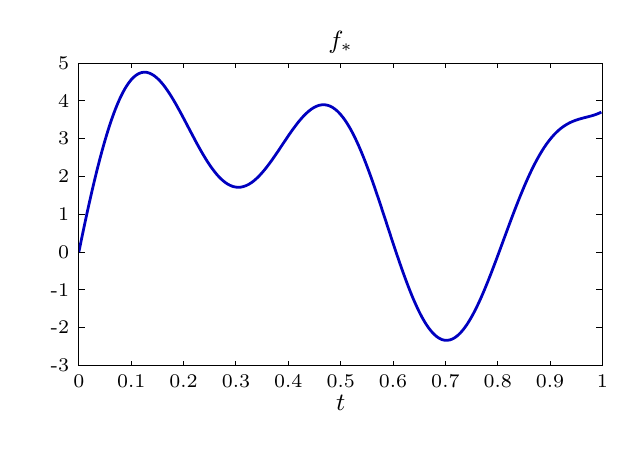
\begin{tikzpicture}[font=\scriptsize]
  % The bounding box matches the physical width of the panel in Figure 5.
  % Text uses explicit LaTeX sizes and is therefore not scaled with the axes.
  \path[use as bounding box] (0,0) rectangle (7.45cm,5cm);
  \begin{scope}[shift={(0.65cm,2.15cm)},x=6.65cm,y=.48cm]
    \draw[line width=.4pt] (0,-3) rectangle (1,5);

    \foreach \x/\lab in {0/0,.1/{0.1},.2/{0.2},.3/{0.3},.4/{0.4},
                            .5/{0.5},.6/{0.6},.7/{0.7},.8/{0.8},.9/{0.9},1/1} {
      \draw[line width=.35pt] (\x,-3) -- +(0,.12);
      \draw[line width=.35pt] (\x,5) -- +(0,-.12);
      \node[anchor=north] at (\x,-3) {\lab};
    }
    \foreach \y in {-3,-2,...,5} {
      \draw[line width=.35pt] (0,\y) -- +(.012,0);
      \draw[line width=.35pt] (1,\y) -- +(-.012,0);
      \node[anchor=east] at (0,\y) {\y};
    }

    \begin{scope}
      \clip (0,-3) rectangle (1,5);
      \draw[blue!75!black,line width=1pt]
        plot[domain=0:1,samples=201,smooth]
        (\x,{64*(\x)^3-96*(\x)^2+36*\x-2+exp(\x)
             +0.8*cos(deg(pi*\x))+2*sin(deg(5*pi*\x+0.1))});
    \end{scope}

    \node at (.5,5.55) {\small $f_*$};
    \node at (.5,-4) {\small $t$};
  \end{scope}
\end{tikzpicture}
\egroup
\pdfpagewidth=\dimexpr\wd0+4pt\relax
\pdfpageheight=\dimexpr\ht0+\dp0+4pt\relax
\hoffset=-1in \voffset=-1in
\shipout\vbox{\kern2pt\hbox{\kern2pt\box0}}
\end{document}
